\documentclass[a4paper, fleqn]{article}
\usepackage[utf8]{inputenc}
\usepackage{amsmath}
\usepackage{amssymb}
\usepackage{caption}
\usepackage{mathtools}
\usepackage{amsfonts}
\usepackage{lastpage}
\usepackage{tikz}
\usepackage{float}
\usepackage{textcomp}
\usetikzlibrary{patterns}
\usepackage{pdfpages}
\usepackage{gauss}
\usepackage{fancyvrb}
\usepackage[table]{colortbl}
\usepackage{fancyhdr}
\usepackage{graphicx}
\usepackage{pdfpages}
\usepackage{enumerate}
\usepackage[margin=2.5 cm]{geometry}

% algorithms
\usepackage{algorithm}      % algorithm float environment
\usepackage[noend]{algpseudocode}  % from algorithmicx; no "end" on functions
\newcommand*\Let[2]{\State #1 $\gets$ #2}
\newtheorem{theorem}{Theorem}
\algnewcommand{\LineComment}[1]{\State \(\sslash\) #1}
\algrenewcommand\algorithmiccomment[1]{\hfill\(\sslash\) #1}
\algrenewcommand\algorithmicrequire{\textbf{Precondition:}}

\setlength\parindent{0pt}
\setlength\mathindent{75pt}

\definecolor{listinggray}{gray}{0.9}
\usepackage{listings}
\lstset{
	language=,
	literate=
		{æ}{{\ae}}1
		{ø}{{\o}}1
		{å}{{\aa}}1
		{Æ}{{\AE}}1
		{Ø}{{\O}}1
		{Å}{{\AA}}1,
	backgroundcolor=\color{listinggray},
	tabsize=3,
	rulecolor=,
	basicstyle=\scriptsize,
	upquote=true,
	aboveskip={0.2\baselineskip},
	columns=fixed,
	showstringspaces=false,
	extendedchars=true,
	breaklines=true,
	prebreak =\raisebox{0ex}[0ex][0ex]{\ensuremath{\hookleftarrow}},
	frame=single,
	showtabs=false,
	showspaces=false,
	showlines=true,
	showstringspaces=false,
	identifierstyle=\ttfamily,
	keywordstyle=\color[rgb]{0,0,1},
	commentstyle=\color[rgb]{0.133,0.545,0.133},
	stringstyle=\color[rgb]{0.627,0.126,0.941},
  moredelim=**[is][\color{blue}]{@}{@},
}

\lstdefinestyle{base}{
  emptylines=1,
  breaklines=true,
  basicstyle=\ttfamily\color{black},
}

\pagestyle{fancy}
\def\checkmark{\tikz\fill[scale=0.4](0,.35) -- (.25,0) -- (1,.7) -- (.25,.15) -- cycle;}
\newcommand*\circled[1]{\tikz[baseline=(char.base)]{
            \node[shape=circle,draw,inner sep=2pt] (char) {#1};}}
\newcommand*\squared[1]{%
  \tikz[baseline=(R.base)]\node[draw,rectangle,inner sep=0.5pt](R) {#1};\!}
\newcommand{\comment}[1]{%
  \text{\phantom{(#1)}} \tag{#1}}
\newcommand\vgap{\vskip 0.1cm}
\def\el{[\![}
\def\er{]\!]}
\def\dpip{|\!|}
\def\MeanN{\frac{1}{N}\sum^N_{n=1}}
\cfoot{Page \thepage\ of \pageref{LastPage}}
\DeclareGraphicsExtensions{.pdf,.png,.jpg}
\author{Nikolaj Dybdahl Rathcke (Student ID: 74763954)}
\title{Cryptography and Coding Theory  \\ Assignment 4}
\lhead{Cryptography and Coding Theory}
\rhead{Assignment 4}

\begin{document}

%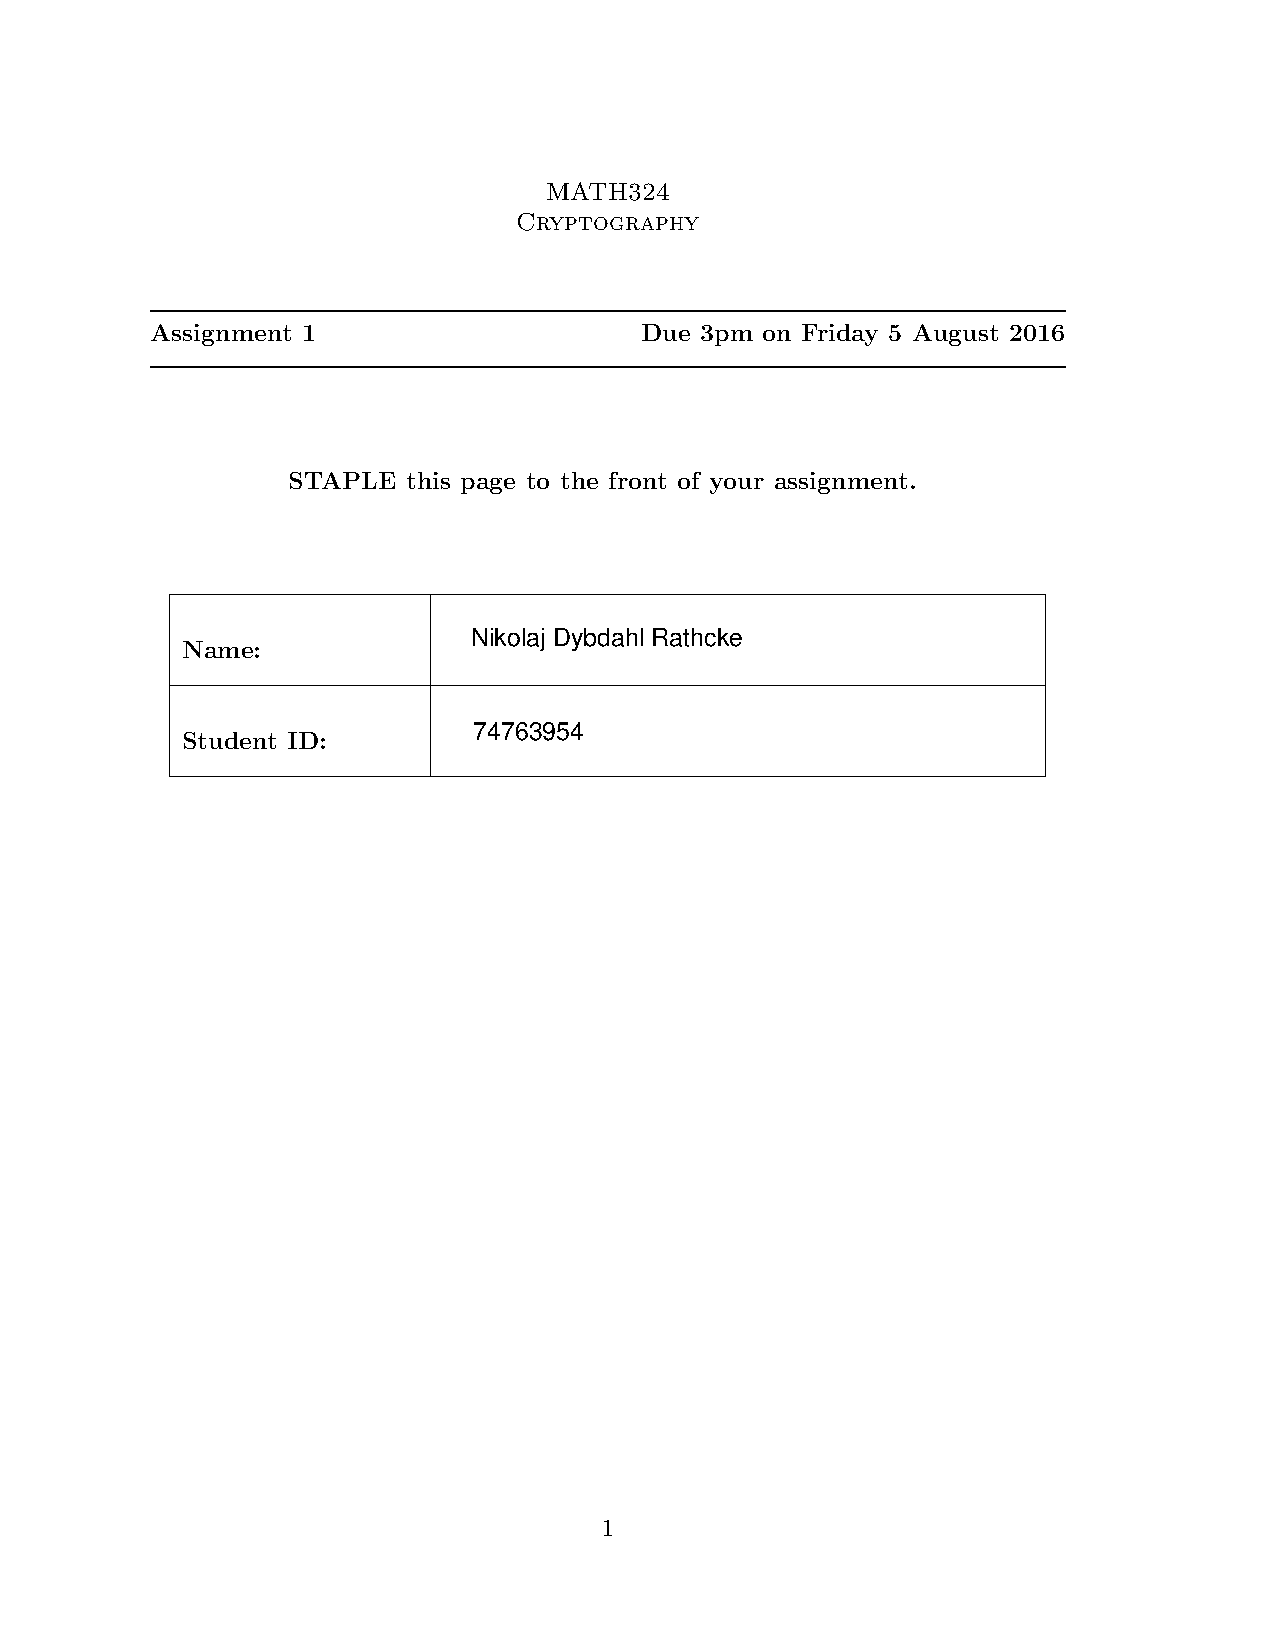
\includepdf[pages=1]{title.pdf}

\section*{Question 1}
\subsection*{(a)}
We have that $n=6$ and $q=2$, so we need to show that $C$ is a subspace of $V(6,2)$. This
is true if and only if:
\begin{enumerate}
  \item The zero vector is in $C$.
  \item For $u,v\in C$, then $u+v\in C$.
  \item For $u\in C$ and scalar $c\in F_2$, then $cu\in C$.
\end{enumerate}
Obviously, criterion $1$ holds as $C$ contains the element $000000$. \\
For the second criterion, consider two codewords $u$ and $v$ of the form
$a_1b_1c_1x_1y_1z_1$ and $a_2b_2c_2x_2y_2z_2$. Since $C$ contains all $2^3$ combinations
of $a,b,c$, that means the sum of the is the codeword with the prefix $a_3b_3c_3$, where $a_3=a_1+a_2$, $b_3=b_1+b_2$ and $c_3=c_1+c_2$. We also have that $x_3\equiv (a_1+a_2)+(b_1+b_2)\equiv
a_3+b_3$ (mod $2$). Likewise $y_3\equiv a_3+c_3$ and $z_3\equiv b_3+c_3$, so we have that
$u+v\in C$. \\
The last one holds as well, since for a $c=0$ and any $u$, then $cu=000000$, which is in
$C$. For $c=1$ and $u\in C$, then clearly $cu=u\in C$. \\
\\
The code $C$ has generator matrix:
\begin{align*}
  \begin{pmatrix}
    1 & 0 & 0 & 1 & 1 & 0 \\
    0 & 1 & 0 & 1 & 0 & 1 \\
    0 & 0 & 1 & 0 & 1 & 1
  \end{pmatrix}
\end{align*}
called $G$.

\subsection*{(c)}
The coset is:
\begin{align*}
  100001+C &= 100001\ \ 101010\ \ 110100\ \ 111111\ \ 000111\ \ 001100\ \ 010010\ \ 011001
\end{align*}

\subsection*{(d)}
We would be able to decode $110101$ correctly. This is because it has distance $1$ to the
codeword $010101$ in $C$. Since any other codeword in $C$ must have distance $\geq 2$ (as
minimum distance in $C$ is $3$) to it, it will always be in the column for $010101$. \\
However, for $011001$, it has minimal distance $2$ to the codewords $001011$, $010101$
and $111000$ - all in $C$. Therefore, depending on the what coset leaders are picked, it
could fall in the columns of any of these. \\
This comes down to the problem of how many errors $C$ can correct since it is nearest
neighbour decoding. This is only $\lfloor \frac{d(C)-1}{2}\rfloor=1$ error.

\section*{Question 2}
\subsection*{(a)}
We have $n=8$. To find the dimension $k$, we need to stack the codewords as rows of a
matrix and perform row reducing:
\begin{align*}
  \begin{bmatrix}
    0 & 0 & 0 & 0 & 0 & 0 & 0 & 0 \\
    0 & 1 & 1 & 0 & 1 & 1 & 1 & 1 \\
    1 & 1 & 0 & 1 & 1 & 0 & 0 & 0 \\
    1 & 1 & 1 & 1 & 1 & 1 & 0 & 1 \\
    1 & 0 & 0 & 1 & 0 & 0 & 1 & 0 \\
    0 & 0 & 1 & 0 & 0 & 1 & 0 & 1 \\
    0 & 1 & 0 & 0 & 1 & 0 & 1 & 0 \\
    1 & 0 & 1 & 1 & 0 & 1 & 1 & 1
  \end{bmatrix}\xrightarrow{\mbox{Row reduction}}
  \begin{bmatrix}
    1 & 0 & 0 & 1 & 0 & 0 & 1 & 0 \\
    0 & 1 & 0 & 0 & 1 & 0 & 1 & 0 \\
    0 & 0 & 1 & 0 & 0 & 1 & 0 & 1 \\
    0 & 0 & 0 & 0 & 0 & 0 & 0 & 0 \\
    0 & 0 & 0 & 0 & 0 & 0 & 0 & 0 \\
    0 & 0 & 0 & 0 & 0 & 0 & 0 & 0 \\
    0 & 0 & 0 & 0 & 0 & 0 & 0 & 0 \\
    0 & 0 & 0 & 0 & 0 & 0 & 0 & 0
  \end{bmatrix}
\end{align*}
The dimension $k$ is then the number non-zero rows, so $k=3$ (row reduction is done over
$GF(2)$ - we would $k=4$ if not). Lastly, the distance $d$ is
the minimum weight of the non-zero codewords, which in this case means $d=3$. \\
So we have $n=8$, $k=3$ and $d=3$. This means we have $n-k=5$ bits of redundancy.

\subsection*{(b)}
If we take the matrix above on reduced row echelon form and remove the rows that are
zero, we get one generator $G_1$:
\begin{align*}
  G_1 &=
    \begin{bmatrix}
    1 & 0 & 0 & 1 & 0 & 0 & 1 & 0 \\
    0 & 1 & 0 & 0 & 1 & 0 & 1 & 0 \\
    0 & 0 & 1 & 0 & 0 & 1 & 0 & 1
  \end{bmatrix}
\end{align*}
Which is on standard coding form. Another generator, $G_2$, not on standard coding form
is easily obtained by exchanging column $2$ and column $7$:
\begin{align*}
  G_2 &=
    \begin{bmatrix}
    1 & 1 & 0 & 1 & 0 & 0 & 0 & 0 \\
    0 & 1 & 0 & 0 & 1 & 0 & 1 & 0 \\
    0 & 0 & 1 & 0 & 0 & 1 & 0 & 1
  \end{bmatrix}
\end{align*}
So the first three columns is not the identity matrix $I_3$.

\subsection*{(c)}
The generator $G_1$ encodes a message $abc$ as $abcvwxyz$, where $abc=vwx$ (repetition
code), $c=z$ (bit repeated twice) and $y\equiv a+b$ (mod $2$).

\subsection*{(d)}
The parity check matrix $H$ of $G_1=[I_k|A]$ is given by:
\begin{align*}
  H&=[-A_{(n-k)\times k}^T|I_{n-k}]=
  \begin{bmatrix}
    1 & 0 & 0 & 1 & 0 & 0 & 0 & 0 \\
    0 & 1 & 0 & 0 & 1 & 0 & 0 & 0 \\
    0 & 0 & 1 & 0 & 0 & 1 & 0 & 0 \\
    1 & 1 & 0 & 0 & 0 & 0 & 1 & 0 \\
    0 & 0 & 1 & 0 & 0 & 0 & 0 & 1
  \end{bmatrix}
\end{align*}
Which is ia $5$ by $8$ matrix.



\end{document}
